\section{Realios mašinos modelis}
	\subsection{Realios mašinos brėžinys}
	\begin{flushleft}
	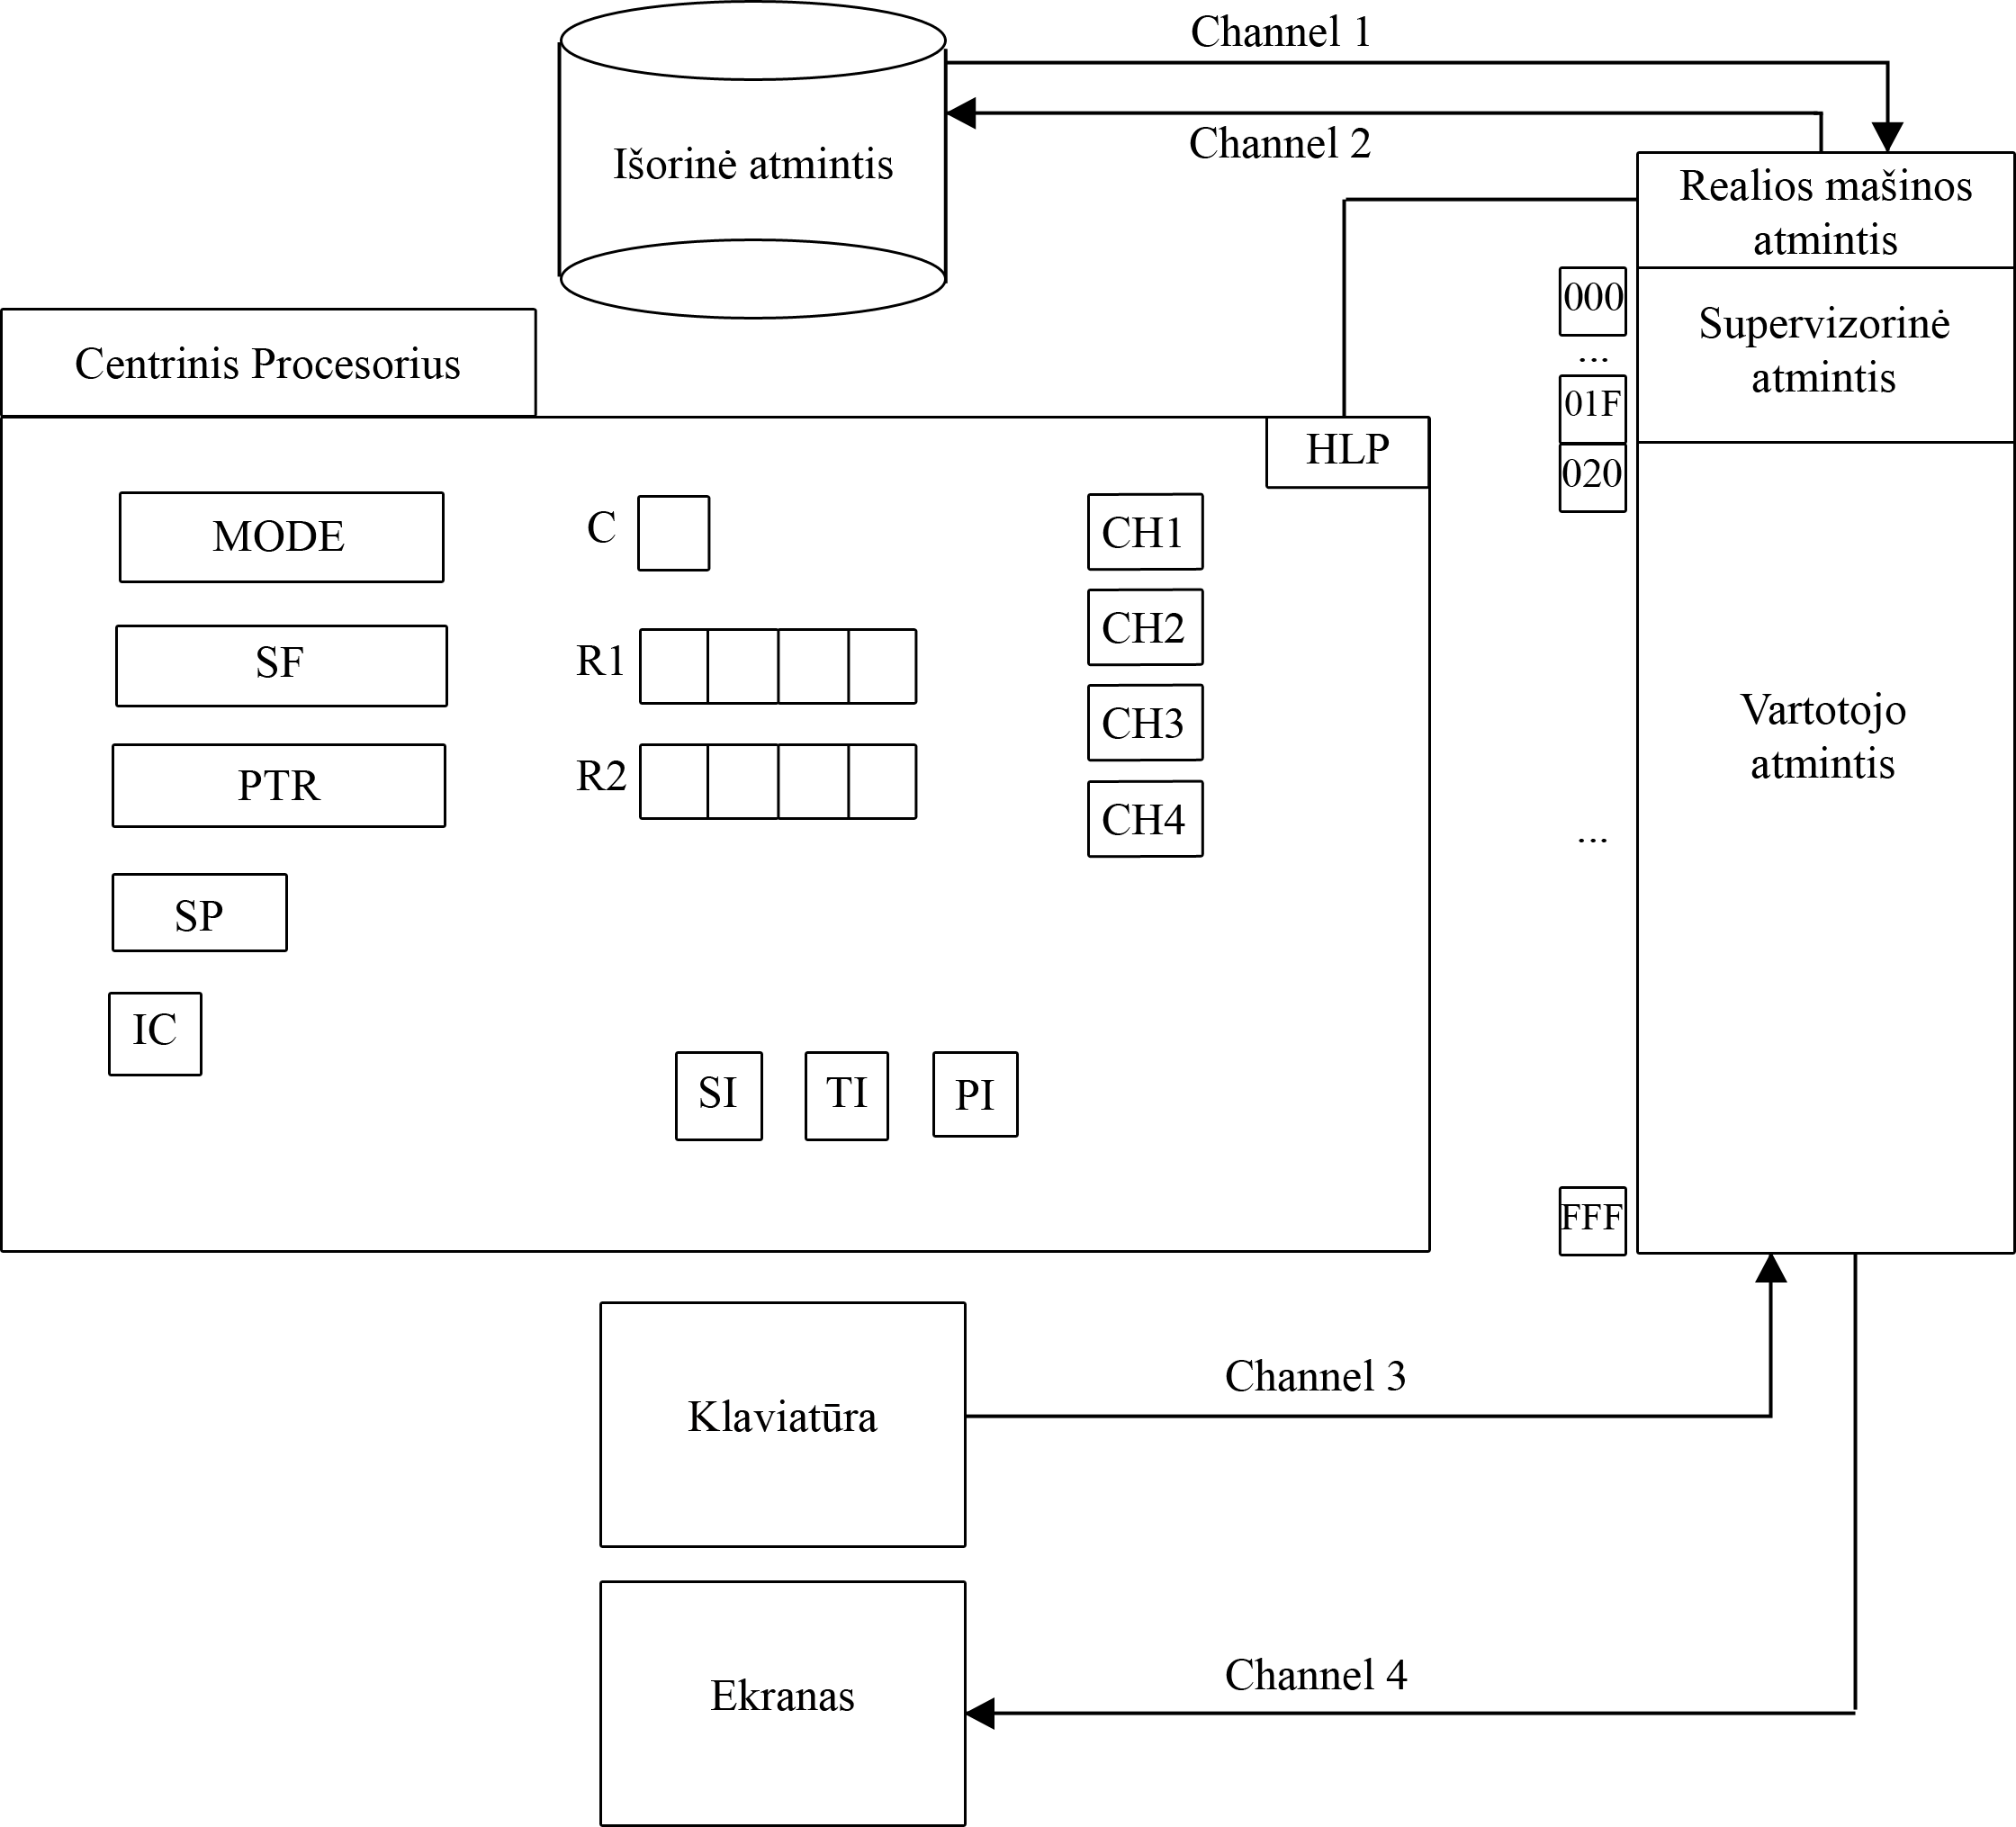
\includegraphics[scale=0.9]{OSv1.png}
	\end{flushleft}
	\subsection{Realios mašinos registrai}
	\begin{enumerate}
	\item HLP - bet kuris aukšto lygio kalbos procesorius. Vartotojo režime HLP vykdo užduoties programą.
	\item MODE - realios mašinos rėžimo registras. Dydis - 1 baitas. Jei reikšmė 0, dirbama supervizoriaus rėžimu, jei reikšmė nėra 0, tada dirbama vartotojo rėžimu.
	\item SF - požymių registras. Dydis - 1 baitas. Parodo procesoriaus būseną po aritmetinio veiksmo.\\
	Požymių registro struktūra: X X X X X CF ZF OF
	\begin{itemize}
		\item X - nenaudojamas.
		\item CF - carry flag. Rezultatas netilpo į skaičiaus be ženklo rėžius.
		\item ZF - zero flag. Rezultatas yra nulis.
		\item OF - overflow flag. Rezultatas netilpo į skaičiaus su ženklu rėžius.
	\end{itemize}
	\item PTR - puslapių lentelės registras. Dydis - 2 baitai. Vyresnysis baitas saugo puslapių lentelės bloko numerį, jaunesnysis baitas saugo puslapių lentelės dydį.
	\item SP - steko rodyklė. Dydis - 1 baitas. Rodo į virtualios mašinos steko viršūnę.
	\item IC - instrukcijų skaitliukas. Dydis - 1 baitas. Rodo virtualios mašinos einamąją instrukciją.
	\item C - loginis trigeris. Dydis - 1 baitas. 0 yra false, visa kita yra true.
	\item R1, R2 - bendros paskirties registrai. Dydis - po 4 baitus. Skirti atlikti komandoms.
	\item Kanalų registrai. Dydis - po 1 baitą.
	\begin{itemize}
		\item CH1 - registras rodantis ar yra atliekamas persiuntimas iš išorinės atminties į realią atmintį.
		\item CH2 - registras rodantis ar yra atliekamas persiuntimas iš realios atminties į išorinę atmintį.
		\item CH3 - registras rodantis ar atliekamas įvedimas iš klaviatūros.
		\item CH4 - registras rodantis ar atliekamas išvedimas į ekraną.
	\end{itemize}
	\item SI - supervizoriaus pertraukimų registras. Dydis - 1 baitas. 
	\item PI - programinių pertraukimų registras. Dydis - 1 baitas.
	\item TI - taimerio registras. Dydis - 1 baitas.
	
	\end{enumerate}	
	
	\subsection{Taimerio mechanizmas}
	Po kiekvienos įvykdytos komandos taimerio registras yra sumažinamas vienetu. Pradinę taimerio reikšmę gali nustatyti vartotojas, tačiau numatytoji reikšmė yra 10.
	
	Kai šio registro reikšmė pasiekia nulį, iškviečiamas supervizorinis taimerio pertraukimas. Įvykdžius taimerio pertraukimo apdorojimo procedūrą, taimerio registro reikšmė vėl tampa 10.
	
	\subsection{Supervizoriniai pertraukimai}
	Supervizoriniai pertraukimai yra iškviečiami tuomet, kai SI registras nėra lygus nuliui arba TI registras yra lygus nuliui.
	
	Pertraukimai pagal SI registro reikšmę:
	\begin{itemize}
	\item 0 - jokio pertraukimo.
	\item 1 - Full stack. Kyla, kai SP reikšmė tampa F. Naudojama swapingo mechanizmui.
	\item 2 - Empty stack. Kyla, kai stekas tampa tuščiu. Naudojama swapingo mechanizmui.
	\item 3 - HALT. Programa baigė darbą. 
	\end{itemize}
	
	\subsection{Programiniai pertraukimai}
	Programiniai pertraukimai yra iškviečiami tuomet, kai PI registras nėra lygus nuliui.
	
	Pertraukimai pagal PI registro reikšmę:
	\begin{itemize}
	\item 0 - jokio pertraukimo.
	\item 1 - Undefined operation code. Neteisingas operacijos kodas.
	\item 2 - Undefined address. Neteisingas adresas.
	\item 3 - Incorrect assignment. Neteisingas priskyrimas.
	\item 4 - Input. Įvedimas iš klaviatūros.
	\item 5 - Output. Išvedimas į ekraną.
	\end{itemize}
	
	\subsection{Realios mašinos rėžimai}
	Reali mašina gali vykdyti darbą dvejais rėžimais: supervizoriaus arba vartotojo. 
	
	Supervizoriaus rėžimu programa bus vykdoma nuo pradžios iki galo, ją nutraukti gali tik pertraukimai. Visi realios mašinos resusrsai yra prieinami.
	
	Vortotojo rėžimu programa gali vykti kelios programos vienu metu, po kiekvieno veiksmo taimeris mažinamas ir kai jis pasiekia nulį, toliau procesoriaus darbą nustato prioritetų automatas. Prieinama atmintis yra tik ta, kurią išskyrė procesorius.
	
	\subsection{Puslapių transliacija}
	Puslapių transliavimo mechanizmas naudojamas, tam, kad galėtumę susieti virtualią ir realią atmintis. registre PTR bus laikomas puslapiavimo lentelės bloko adresas, kurio kiekviename žodyje bus laikomas virtualios mašinos puslapio takelio adresas. 
	\(a_0\) ir \(a_1\) naudojami naudojamas gauti puslapių leneltės adresą, naudojama formulė yra tokia:\\ \(10 * a_0 + a_1\)
	
	Dviženklis adresas \(x_0\), \(x_1\) realiojoje mašinoje apskaičiuojamas taip:\\ \(10 * [10 *(10 * a_0 + a_1) + x_0] + x_1\)  
	\subsection{Swapingas}
	Kai steke pritrūksta vietos, dalis steko turinio yra perkeliamas į išorinę atmintį.
	
	Kai stekas tampa tuščias, į jį grąžinami duomenys iš išorinės atminties, jei jų yra.
	
	Kiekvienai programai yra sukuriamas laikinas failas, kur ir bus dedamas stekas, jei to prireiks. Programai pasibaigus šis failas bus ištrinamas.
	
	\subsection{Įvedimas ir išvedimas}
	Kadangi projektuojama OS yra interaktyvi, vartotojas gali įvesti komandas ir/ar duomenis ir taip reguliuoti realios mašinos darbą ir matyti šių komandų rezultatus.
	
	Įvedimo įrenginys - klaviatūra. Suvedama komanda arba jos duomenys ir paspaudžiamas mygtukas ENTER, kad būtų paleidžiamas arba pratęsiamas jos vykdymas.
	
	Išvedimo įrenginys - ekranas. Įvykdytų komandų rezultatai gali būti išvedami į ekraną.
	
	\subsection{Atminties įrenginiai}
	\textbf{Išorinė atmintis} - kietasis diskas. Jame duomenys bus išsaugoti net ir išjungus realią mašiną.
	
	\textbf{Realios mašinos atmintis} - atmintis esanti realioje mašinoje. Ji suskirstyta į 16 blokų po 16 žodžių, vieno žodžio dydis yra 32 bitai. Ją toliau skirstome į supervizorinę ir vartotojo atmintį:
	\begin{itemize}
	\item \textbf{Supervizorinė atmintis} - 2 blokai išskirti realios mašinos atminties pradžioje. Jie nėra prieinami vartotojui.
	\item \textbf{Vartotojo atmintis} - Visa likusi realios mašinos atmintis. Ją galima skirstyti virtualioms mašinoms.
	\end{itemize}
	
	\subsection{Išorinė atmintis}
	Išorinė atmintis bus realizuojama failu kietajame diske. Darbą su ja vykdys HLP.
\clearpage